\documentclass[border=1cm]{standalone}

\usepackage{tikz}

\usetikzlibrary{3d,calc,intersections}

\begin{document}
    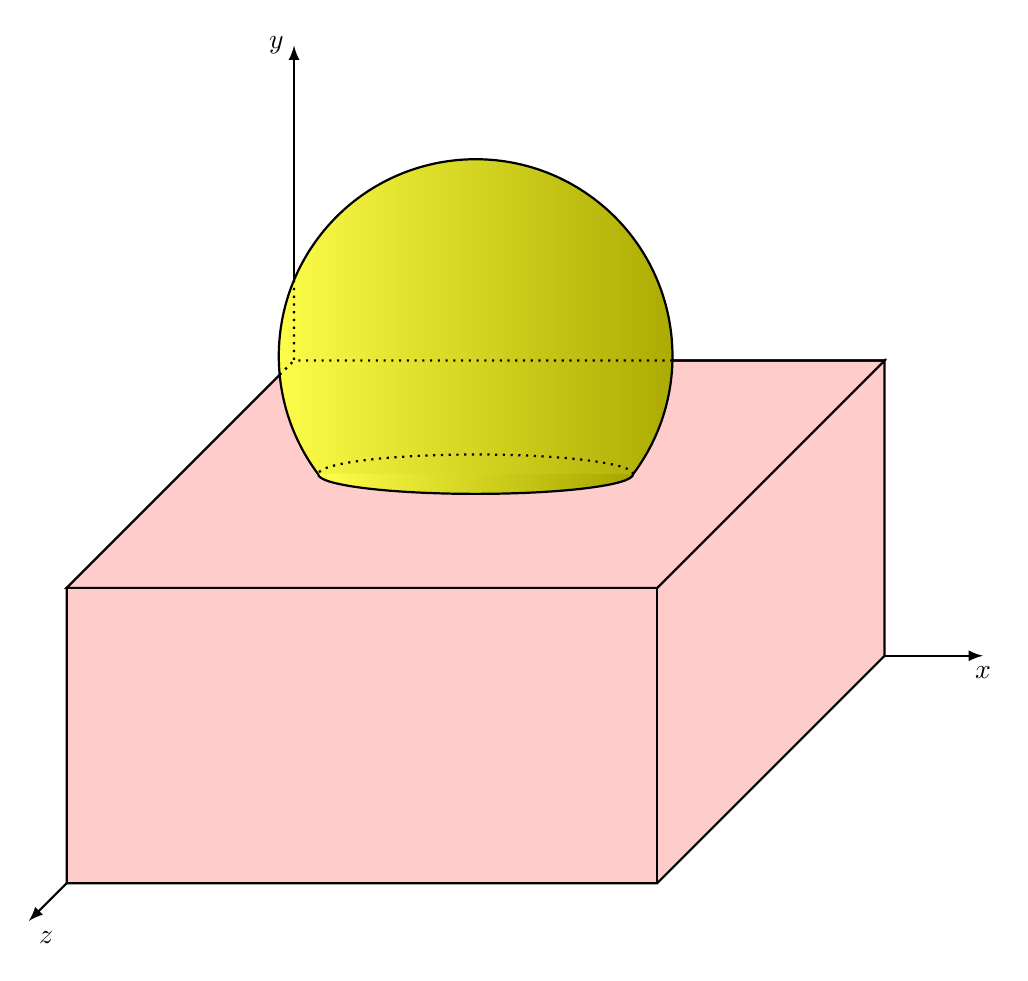
\begin{tikzpicture}[scale=0.25, thick]
        \draw[->, >=latex] (30,0)--(35,0) node[below]{$x$};
        \draw[->, >=latex] (0,15)--(0,31) node[left]{$y$};
        \draw[->, >=latex] (0,0,30)--(0,0,35) node[below right]{$z$};

        \draw[fill=red!20] (0,15,30)--(0,0,30)--(30,0,30)--(30,0,0)--(30,15)--(30,15,30)--cycle;
            (0,15,0)--(0,15,30);
        \draw (30,0,30)--(30,15,30);
        \draw[fill=red!20](0,15)--(30,15)--(30,15,30)--(0,15,30)--cycle;
        \draw[name path=esfera, left color=yellow!70, right color=olive!70] 
            ($(15,21,15) + ({-atan(6/8)}:10cm)$) arc [start angle={-atan(6/8)}, end angle={180+atan(6/8)}, radius=10cm];
        \draw[left color=yellow!70, right color=olive!70] (15-8,15,15) arc [start angle=-180, end angle=0, x radius=8, y radius=1];
        \draw[dotted] (15+8,15,15) arc [start angle=0, end angle=180, x radius=8, y radius=1];
        \path[name path=aresta] (30,15)--(0,15);
        \path[name intersections={of=esfera and aresta}];
        \draw (intersection-1)--(30,15);
        \draw[dotted] (intersection-1)--(0,15);
        \path[name path=aresta1] (0,0)--(0,31);
        \path[name intersections={of=esfera and aresta1}];
        \draw[dotted] (intersection-2)--(0,15);
        \path[name path=aresta2] (0,15)--(0,15,30);
        \path[name intersections={of=esfera and aresta2}];
        \draw[dotted] (intersection-1)--(0,15);
        
    \end{tikzpicture}
\end{document}


%C.A.)
% 31-15=16
%
% 8²+(16-r)²=r^2
% 64 + 256-32r+r^2=r^2<=>r=320/32<=> r=10